
\section{Methodology}

As shown in Figure~\ref{main_framework_meta_transf_hard_task},  our method consists of three phases.
%
First, we train a DNN on large-scale data, e.g. on miniImageNet ($64$-class, $600$-shot)~\cite{VinyalsBLKW16}, and then fix the low-level layers as Feature Extractor (Section~\ref{sec_large_scale_pretrain}). 
%
Second, in the meta-transfer learning phase, MTL learns the \emph{Scaling} and \emph{Shifting} (\emph{SS}) parameters for the Feature Extractor neurons, enabling fast adaptation to few-shot tasks (Section~\ref{sec_meta_transfer}).
%
For improved overall learning, we use our HT meta-batch strategy  (Section~\ref{sec_HT}).
The training steps are detailed in Algorithm~\ref{alg_overall} in Section~\ref{sec_alg}.
%
Finally, the typical meta-test phase is performed, as introduced in Section~\ref{sec_preli}.

%%%
\subsection{DNN training on large-scale data}
\label{sec_large_scale_pretrain}

This phase is similar to the classic pre-training stage as, e.g., pre-training on Imagenet for object recognition~\cite{Russakovsky2015}.
%
%
Here, we do not consider data/domain adaptation from other datasets, and  pre-train on readily available data of few-shot learning benchmarks, allowing for fair comparison with other few-shot learning methods.
%
Specifically, for a particular few-shot dataset, we merge all-class data $\mathcal{D}$ for pre-training.
%
For instance, for miniImageNet~\cite{VinyalsBLKW16}, there are totally $64$ classes in the training split of $\mathcal{D}$ and each class contains $600$ samples used to pre-train a $64$-class classifier.
%

We first randomly initialize a feature extractor $\Theta$ (e.g. CONV layers in ResNets~\cite{HeZRS16}) and a classifier $\theta$ (e.g. the last FC layer in ResNets~\cite{HeZRS16}), and then optimize them by gradient descent as follows,
\begin{equation}\label{eq_large_scale_update}
 [\Theta; \theta] =: [\Theta; \theta] - \alpha\nabla\mathcal{L}_{\mathcal{D}}\big([\Theta; \theta]\big),
\end{equation}
where $\mathcal{L}$ denotes the following empirical loss,
\begin{equation}\label{eq_large_scale_loss}
    \mathcal{L}_{\mathcal{D}}\big([\Theta; \theta]\big) = \frac{1}{|\mathcal{D}|}\sum_{(x,y)\in \mathcal{D}}l\big(f_{[\Theta; \theta]}(x), y\big),
\end{equation}
e.g. cross-entropy loss, and $\alpha$ denotes the learning rate. 
%
In this phase, the feature extractor $\Theta$ is learned. It will be frozen in the following meta-training and meta-test phases, as shown in Figure~\ref{main_framework_meta_transf_hard_task}. 
%
The learned classifier $\theta$ will be discarded, because subsequent few-shot tasks contain different classification objectives, e.g. $5$-class instead of $64$-class classification for miniImageNet~\cite{VinyalsBLKW16}.
%%%%%%%%%%%%%%%%%%%%%%%%%%%%%%%%%%%%%%%%%%%%%%%%%%%%%%%%%

\subsection{Meta-transfer learning (MTL)}
\label{sec_meta_transfer}

As shown in Figure~\ref{main_framework_meta_transf_hard_task}(b), our proposed meta-transfer learning (MTL) method optimizes the meta operations \emph{Scaling} and \emph{Shifting} (\emph{SS}) through HT meta-batch training (Section~\ref{sec_HT}). 
%
Figure~\ref{main_framework_SS_FT} visualizes the difference of updating through \emph{SS} and \emph{FT}.
\emph{SS} operations, denoted as $\Phi_{S_1}$ and $\Phi_{S_2}$, do not change the frozen neuron weights of $\Theta$ during learning, while \emph{FT} updates the complete $\Theta$. 
%

In the following, we detail the \emph{SS} operations.
%
%
Given a task $\mathcal{T}$, the loss of $\mathcal{T}^{(tr)}$ is used to optimize the current base-learner (classifier) $\theta'$ by gradient descent:
\begin{equation}\label{eq_base_classifier}
  \theta' \gets \theta - \beta\nabla_{\theta}\mathcal{L}_{\mathcal{T}^{(tr)}}\big([\Theta; \theta], \Phi_{S_{\{1,2\}}}\big),
\end{equation}
which is different to Eq.~\ref{eq_large_scale_update}, as we do not update $\Theta$. 
Note that here $\theta$ is different to the one from the previous phase, the large-scale classifier $\theta$ in Eq.~\ref{eq_large_scale_update}. 
%
This $\theta$ concerns only a few of classes, e.g. 5 classes, to classify each time in a novel few-shot setting. 
%
$\theta'$ corresponds to a temporal classifier only working in the current task, initialized by the $\theta$ optimized for the previous task (see Eq.~\ref{eq_meta_classifier}). 


$\Phi_{S_1}$ is initialized by ones and $\Phi_{S_1}$ by zeros. Then, they are optimized by the test loss of $\mathcal{T}^{(te)}$ as follows,
%
\begin{equation}\label{eq_ss_update}
     \Phi_{S_i} =: \Phi_{S_i} - \gamma\nabla_{\Phi_{S_i}}\mathcal{L}_{\mathcal{T}^{(te)}}\big([\Theta; \theta'], \Phi_{S_{\{1,2\}}}\big).
\end{equation}
%
%
In this step, $\theta$ is updated with the same learning rate $\gamma$ as in Eq.~\ref{eq_ss_update},
\begin{equation}\label{eq_meta_classifier}
  \theta =: \theta - \gamma\nabla_{\theta}\mathcal{L}_{\mathcal{T}^{(te)}}\big([\Theta; \theta'], \Phi_{S_{\{1,2\}}}\big).
\end{equation}
Re-linking to Eq.~\ref{eq_base_classifier}, we note that the above $\theta'$ comes from the last epoch of base-learning on $\mathcal{T}^{(tr)}$.

Next, we describe how we apply $\Phi_{S_{\{1,2\}}}$ to the frozen neurons as shown in Figure~\ref{main_framework_SS_FT}(b). 
Given the trained $\Theta$, for its $l$-th layer containing $K$ neurons, we have $K$ pairs of parameters, respectively as weight and bias, denoted as $\{(W_{i,k}, b_{i,k})\}$. Note that the neuron location $l, k$ will be omitted for readability.
%
Based on MTL, we learn $K$ pairs of scalars $\{\Phi_{S_{\{1,2\}}}\}$. 
%
Assuming $X$ is input, we apply $\{\Phi_{S_{\{1,2\}}}\}$ to $(W, b)$ as
\begin{equation}\label{eq_SS_operation}
    SS(X; W, b; \Phi_{S_{\{1,2\}}}) =(W\odot\Phi_{S_1}) X + (b + \Phi_{S_2}),
\end{equation}
where $\odot$ denotes the element-wise multiplication.

\begin{figure}[t]
  \centering
  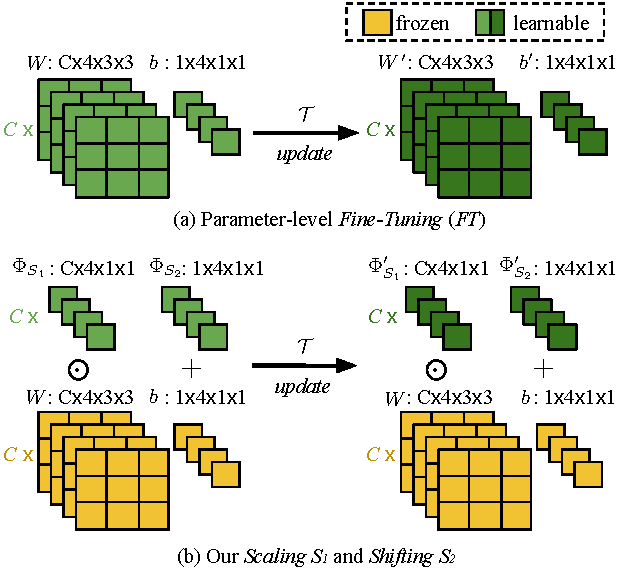
\includegraphics[width=0.99\linewidth]{figures/main_framework_SS_FT.pdf}
     \caption{(a) Parameter-level \emph{Fine-Tuning} (\emph{FT}) is a conventional meta-training operation, e.g. in MAML~\cite{FinnAL17}. Its update works for all neuron parameters, $W$ and $b$.
     (b) Our neuron-level \emph{Scaling} and \emph{Shifting} (\emph{SS}) operations in MTL. They reduce the number of learning parameters and avoid overfitting problems. In addition, they keep large-scale trained parameters (in yellow) frozen, preventing ``catastrophic fogetting''~\cite{LopezPazNIPS17, McCloskey1989}.
    }
  \label{main_framework_SS_FT}
\end{figure}


Taking Figure~\ref{main_framework_SS_FT}(b) as an example of a single $3\times 3$ filter, after \emph{SS} operations, this filter is scaled by $\Phi_{S_1}$ then the feature maps after convolutions are shifted by $\Phi_{S_2}$ in addition to the original bias $b$. 
Detailed steps of \emph{SS} are given in Algorithm~\ref{alg_Meta} in Section~\ref{sec_alg}.
%

Figure~\ref{main_framework_SS_FT}(a) shows a typical parameter-level \emph{Fine-Tuning} (\emph{FT}) operation, which is in the meta optimization phase of our related work MAML~\cite{FinnAL17}.
%
It is obvious that \emph{FT} updates the complete values of $W$ and $b$, and has a large number of parameters, and our \emph{SS} reduces this number to below $\tfrac{2}{9}$ in the example of the figure. 
%


In summary, \emph{SS} can benefit MTL in three aspects.
1) It starts from a strong initialization  based on a large-scale trained DNN, yielding fast convergence for MTL.
2) It does not change DNN weights, thereby avoiding the problem of ``catastrophic forgetting''~\cite{LopezPazNIPS17, McCloskey1989} when learning specific tasks in MTL.
3) It is light-weight, reducing the chance of overfitting of MTL in few-shot scenarios.
%
%



\subsection{Hard task (HT) meta-batch}
\label{sec_HT}

In this section, we introduce a method to schedule hard tasks in meta-training batches. 
%
The conventional meta-batch is composed of randomly sampled tasks, where the randomness implies random difficulties~\cite{FinnAL17}.
In our meta-training pipeline, we intentionally pick up failure cases in each task and re-compose their data to be harder tasks for adverse re-training. 
We aim to force our meta-learner to ``grow up through hardness''. 

\myparagraph{Pipeline.}
Each task $\mathcal{T}$ has two splits, $\mathcal{T}^{(tr)}$ and $\mathcal{T}^{(te)}$, for base-learning and test, respectively.
As shown in Algorithm~\ref{alg_Meta} line 2-5, base-learner is optimized by the loss of $\mathcal{T}^{(tr)}$ (in multiple epochs). \emph{SS} parameters are then optimized by the loss of $\mathcal{T}^{(te)}$ once.
%
We can also get the recognition accuracy of $\mathcal{T}^{(te)}$ for $M$ classes. Then, we choose the lowest accuracy $Acc_m$ to determine the most difficult class-$m$ (also called failure class) in the current task.

%
%
After obtaining all failure classes (indexed by $\{m\}$) from $k$ tasks in current meta-batch $\{\mathcal{T}_{1\sim k}\}$, we re-sample tasks from their data. 
%
Specifically, we assume $p(\mathcal{T}|\{m\})$ is the task distribution, we sample a ``harder'' task $\mathcal{T}^{hard} \in p(\mathcal{T}|\{m\})$.
Two important details are given below.


%
\myparagraph{Choosing hard class-$m$.} We choose the failure class-$m$ from each task by ranking the class-level accuracies instead of fixing a threshold.
%
In a dynamic online setting as ours, it is more sensible to choose the hardest cases based on ranking rather than fixing a threshold ahead of time. 
%

\myparagraph{Two methods of hard tasking using $\{m\}$.}
%
Chosen $\{m\}$, we can re-sample tasks $\mathcal{T}^{hard}$ by (1) directly using the samples of class-$m$ in the current task $\mathcal{T}$, or (2) indirectly using the label of class-$m$ to sample new samples of that class.
In fact, setting (2) considers to include more data variance of class-$m$ and it works better than setting (1) in general. 
%%



%%%%%%%%%%%%%%%%%%%%%%%%%%%%%%%%%%%%%%%%%%%%%%%%%%%%%%%%%
%%%%%%%%%%%%%%%%%%%%%%%%%%%%%%%%%%%%%%%%%%%%%%%%%%%%%%%%%
\subsection{Algorithm}
\label{sec_alg}

Algorithm~\ref{alg_overall} summarizes the training process of two main stages: large-scale DNN training (line 1-5) and meta-transfer learning (line 6-22). HT meta-batch re-sampling and continuous training phases are shown in lines 16-20, for which the failure classes are returned by Algorithm~\ref{alg_Meta}, see line 14.
Algorithm~\ref{alg_Meta} presents the learning process on a single task that includes episode training (lines 2-5) and episode test, i.e. meta-level update (lines 6). In lines 7-11, the recognition rates of all test classes are computed and returned to Algorithm~\ref{alg_overall} (line 14) for hard task sampling.

%%%%%%%%%%%%%%%%%%%%%%%%%%%%%%%%%%%%%%%%%%%%%%%%%%%%%%%%%%%

\begin{algorithm}
\caption{Meta-transfer learning (MTL)}
\label{alg_overall}
\SetAlgoLined
\SetKwInput{KwData}{Input}
\SetKwInput{KwResult}{Output}
 \KwData{Task distribution $p(\mathcal{T})$ and corresponding dataset $\mathcal{D}$, learning rates $\alpha$, $ \beta$ and $\gamma$}
 \KwResult{Feature extractor $\Theta$, base learner $\theta$, \emph{SS} parameters $\Phi_{S_{\{1,2\}}}$}
 Randomly initialize $\Theta$ and $\theta$\;
 \For{samples in $\mathcal{D}$}{
 Evaluate $\mathcal{L}_{\mathcal{D}}([\Theta; \theta])$ by Eq.~\ref{eq_large_scale_loss}\;
 Optimize $\Theta$ and $\theta$ by Eq.~\ref{eq_large_scale_update}\;
 }
  Initialize $\Phi_{S_1}$ by ones, initialize $\Phi_{S_2}$ by zeros\;
  Reset and re-initialize $\theta$ for few-shot tasks\;
%   Randomly initialize $\theta$\;
 \For{meta-batches}{
 Randomly sample tasks $\{\mathcal{T}\}$ from $p(\mathcal{T})$\;
 \While{not done}{
 Sample task $\mathcal{T}_i \in \{\mathcal{T}$\}\;
 Optimize $\Phi_{S_{\{1,2\}}}$ and $\theta$ with $\mathcal{T}_i$ by \textbf{Algorithm}~\ref{alg_Meta}\;
 Get the returned class-$m$ then add it to $\{m\}$\;
 }
 Sample hard tasks $\{\mathcal{T}^{hard}\}$ from $\subseteq p(\mathcal{T}|\{m\})$\;
  \While{not done}{
 Sample task $\mathcal{T}^{hard}_j \in \{\mathcal{T}^{hard}$\} \;
 Optimize $\Phi_{S_{\{1,2\}}}$ and $\theta$ with $\mathcal{T}^{hard}_j$ by \textbf{Algorithm}~\ref{alg_Meta} \;
 }
 Empty $\{m\}$.
 }
\end{algorithm}

%%%%%%%%%%%%%%%%%%%%%%%%%%%%%%%%%%%%%%%%%%%%%%%%%%%%%%%%%%%

%%%%%%%%%%%%%%%%%%%%%%%%%%%%%%%%%%%%%%%%%%%%%%%%%%%%%%%%%%%

\begin{algorithm}
\caption{Detail learning steps within a task $\mathcal{T}$}
\label{alg_Meta}
\SetAlgoLined
\SetKwInput{KwData}{Input}
\SetKwInput{KwResult}{Output}
 \KwData{$\mathcal{T}$, learning rates $ \beta$ and $\gamma$, feature extractor $\Theta$, base learner $\theta$, \emph{SS} parameters $\Phi_{S_{\{1,2\}}}$}
 \KwResult{Updated $\theta$ and $\Phi_{S_{\{1,2\}}}$, 
 the worst classified class-$m$ in $\mathcal{T}$}
 Sample $\mathcal{T}^{(tr)}$ and $\mathcal{T}^{(te)}$ from $\mathcal{T}$ \;
 \For{samples in $\mathcal{T}^{(tr)}$}{
 Evaluate $\mathcal{L}_{\mathcal{T}^{(tr)}}$\;
 Optimize $\theta'$ by Eq.~\ref{eq_base_classifier}\;
 }
 Optimize $\Phi_{S_{\{1,2\}}}$ and $\theta$ by Eq.~\ref{eq_ss_update} and Eq.~\ref{eq_meta_classifier}\;
 \While{not done}{
 Sample class-$k$ in $\mathcal{T}^{(te)}$\;
 Compute $Acc_k$ for $\mathcal{T}^{(te)}$\;
 }
 Return class-$m$ with the lowest accuracy $Acc_m$.
\end{algorithm}
\vspace{-6mm}
%%%%%%%%%%%%%%%%%%%%%%%%%%%%%%%%%%%%%%%%%%%%%%%%%%%%%%%%%%%


